\section{Auswertung}

Die Größenmessung der Gegenstands- und der Bildgröße wurde mit einem Geodreieck durchgeführt.
Die weiteren Messwerte wurden an einem Lineal, welches an der Schiene integriert
ist, abgelesen. Es wird ein Ablesefehler von $\SI{0,05}{\centi\meter}$ angenommen.
Anhand der genommenen Messwerte wird die Linsengleichung \eqref{eqn:Linsengleichung} und das
Abbildungsgesetz \eqref{eqn:Abbildungsgesetz} überprüft.

Damit das Abbildungsgesetz überprüft werden kann, sind die Daten der Messung
der Gegenstands- und der Bildweite verwendet worden.
Die Messdaten sind in Tabelle \ref{tab:bekannte_brennweite} dargestellt.
In den folgenden Gleichungen sind die Mittelwerte der Messung und die dazugehörige
Standardabweichung dargestellt.

\begin{align}
  \label{eqn:B/G}
  \frac{B}{G}=&\SI{56,9(9)}{\centi\meter} \\
  \label{eqn:b/g}
  \left<\frac{b}{g}\right>=&\SI{54,30(9)}{\centi\meter}
\end{align}

\begin{table}
\centering
\caption{Messdaten der ersten Messung. Brennweite der verwendeten Linse ist bekannt ($\SI{10}{\centi\meter}$).}
\label{tab:bekannte_brennweite}
\begin{tabular}{S S S S S}
\toprule
{$g$ in $\si{\centi\meter}$} & {$b$ in $\si{\centi\meter}$} & {Bildgröße $B$} & {Brennweite $f$} & {$\Delta f$}\\
\midrule
15 & 27.80  & \,\,\,\,\,\,\,\,\,\,\,\,\,\,\,\text{--} & 9,74 & 0,02 \\
20 & 18.40  & 2.80 & 9,56 & 0,02 \\
25 & 15.30  & 1.90 & 9,49 & 0,02 \\
30 & 13.85  & 1.45 & 9,47 & 0,02 \\
35 & 13.10  & 1.15 & 9,53 & 0,03 \\
40 & 12.50  & 0.95 & 9,52 & 0,03 \\
45 & 12.05  & \,\,\,\,\,\,\,\,\,\,\,\,\,\,\,\text{--} & 9,50 & 0,03 \\
50 & 11.70  & \,\,\,\,\,\,\,\,\,\,\,\,\,\,\,\text{--} & 9,48 & 0,03 \\
55 & 11.40  & \,\,\,\,\,\,\,\,\,\,\,\,\,\,\,\text{--} & 9,44 & 0,03 \\
60 & 11.25  & \,\,\,\,\,\,\,\,\,\,\,\,\,\,\,\text{--} & 9,47 & 0,04 \\
\bottomrule
\end{tabular}
\end{table}


Die Fehler der Größen in \ref{tab:bekannte_brennweite} haben alle den Ablesefehler
$\SI{0,05}{\centi\meter}$.

Die Werte von $g$ und $b$ wurden in \eqref{eqn:Linsengleichung} eingesetzt und es wurde der Mittelwert der Brennweite bestimmt. Die Brennweite der Linse ist vom Hersteller mit $\SI{10}{\centi\meter}$
angegeben.

\begin{description}
  \centering
  \item[$<f_1>\ua{gemessen}=$]\SI{9,525(9)}{\centi\meter}
\end{description}

Die Verbindungsgereaden zu den Wertepaaren $(g_i|b_i)$ der Linse mit bekannter
Brennweite sind in \ref{fig:brennweite_bekannt}
dargestellt.

\begin{figure}
  \centering
  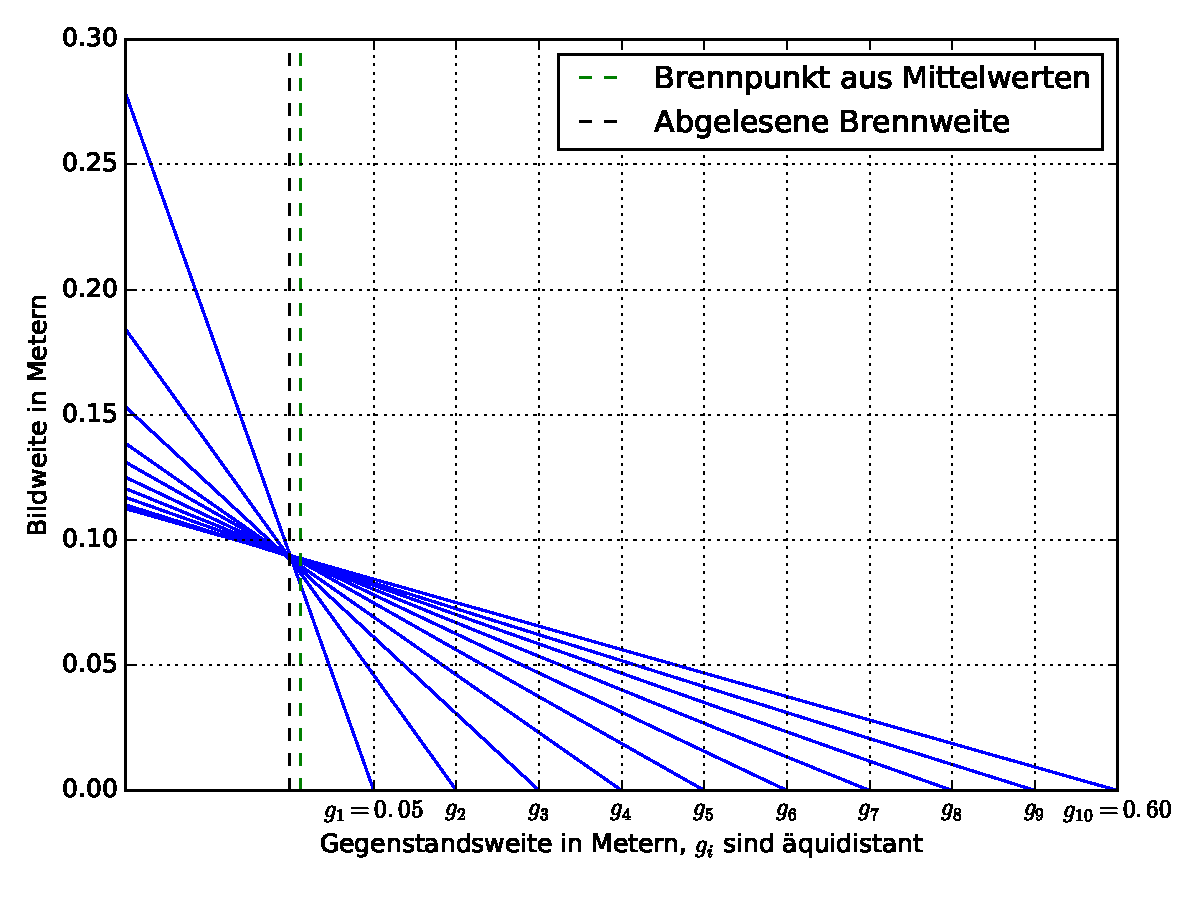
\includegraphics[width=\textwidth]{Pics/Messung1_brennnweite_bekannt.pdf}
  \caption{Wertepaare $(g_i|b_i)$ aufgetragen. Zudem ist der Mittelwert der gemessenen Brennweite sowie der abgelesene Schnittpunkt der Geraden eingetragen.}
  \label{fig:brennweite_bekannt}
\end{figure}

Der Schnittpunkt der Geraden im Diagramm \ref{fig:brennweite_bekannt}
ist mit Hilfe des Mauscoursers abgelesen worden. Der Ablesefehler wird mit
$\SI{0,3}{\centi\meter}$ angegeben.
Der Schnittpunkt hat einen Wert von $S_1 = (\num{9,9(3)}|\num{9,4(3)})$.
Die Angaben sind in Centimetern. Die Fehler wurden als Ablesefehler des Diagrammes angenommen.

Des Weiteren wurde die Brennweite einer unbekannten Linse bestimmt.
Es wurde das gleiche Verfahren wie bei der Messung der Linse mit bekannter
Brennweite verwendet.
Die Messdaten sind in Tabelle \ref{tab:unbekannte_brennweite} dargestellt.

\begin{description}
  \centering
  \item[$<f_2>\ua{gemessen}=$]\SI{8,383(9)}{\centi\meter}
\end{description}

Das Diagramm \ref{fig:unbekannte_brennweite} zeigt die Verbindungsgeraden
der gemessenenen Wertepaare  $(g_i|b_i)$.

\begin{figure}
  \centering
  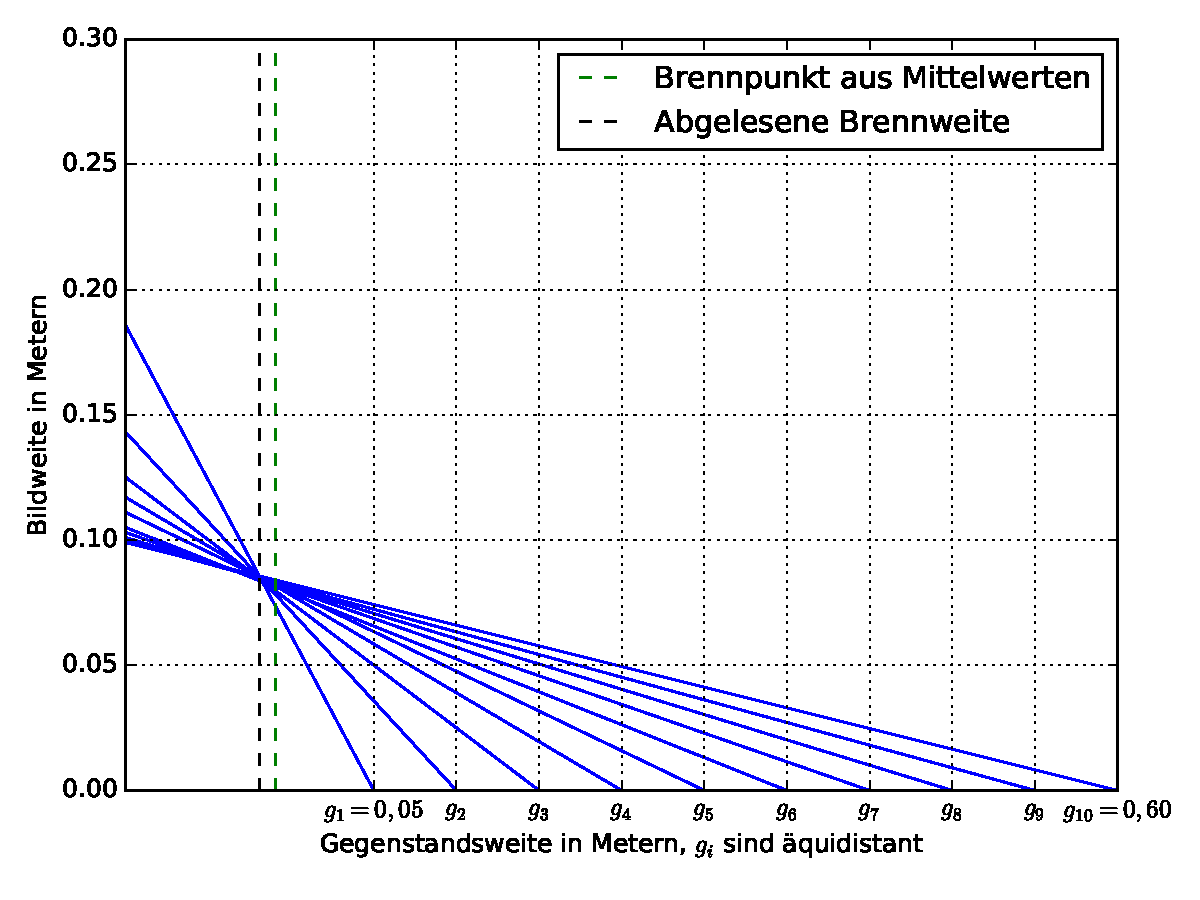
\includegraphics[width=\textwidth]{Pics/Messung2_unbekannte_brennweite.pdf}
  \caption{Wertepaare $(g_i|b_i)$ aufgetragen. Zudem ist der Mittelwert der gemessenen Brennweite, sowie der abgelesene Schnittpunkt der Geraden eingetragen.}
  \label{fig:unbekannte_brennweite}
\end{figure}

Der abgelesene Schnittpunkt ist gegeben mit $S_2 =
(\num{8,1(3)}|\num{8,4(3)})$. Die Angaben sind in Centimetern.
Es wird ein Ablesefehler von $0,03\su{cm}$ angenommen.

\begin{table}
\centering
\caption{Messdaten der Linse mit unbekannter Brennweite.}
\label{tab:unbekannte_brennweite}
\begin{tabular}{S S}
\toprule
{$g$ in $\si{\centi\meter}$} & {$b$ in $\si{\centi\meter}$} \\
\midrule
15 & 18.55 \\
20 & 14.30 \\
25 & 12.50 \\
30 & 11.70 \\
35 & 11.10 \\
40 & 10.50 \\
45 & 10.30 \\
50 & 10.10 \\
55 & 9.95  \\
60 & 9.90  \\
\bottomrule
\end{tabular}
\end{table}


Die Messgrößen in Tabelle \ref{tab:unbekannte_brennweite} haben alle den Ablesefehler
$\SI{0,05}{\centi\meter}$.

\subsection{Bestimmung der Brennweite nach Bessel}

Die Messdaten der Messung sind in Tabelle \ref{tab:bessel} dargestellt.
Damit der Datensatz größer ist, werden die Messdaten
von $b_1, g_1$ und $b_2, g_2$ verwendet. Theoretisch sind $b_1 = g_2$
und $b_2 = g_1$ identisch.

Die Mittelwerte der Messdaten wurden in die Formel \eqref{eqn:Bessel} eigetragen.
Daraus ergibt sich die folgende Brennweite.

\begin{equation}
  \centering
  \label{eqn:bessel_ergebnis}
  f\ua{Bessel}= \SI{9,67}{\centi\meter}
\end{equation}

Der Fehler von \eqref{eqn:bessel_ergebnis} ist bezüglich der Messgenauigkeit
vernachlässigbar klein und wird daher weggelassen.

\begin{table}
\centering
\caption{Messdaten der Methode nach Bessel}
\label{tab:bessel}
\begin{tabular}{S S S S S S }
\toprule
{$e$ in $\si{\centi\meter}$} & {Fehler $e$} & {$g_1$ in $\si{\centi\meter}$} & {Fehler $g_1$} & {$g_2$ in $\si{\centi\meter}$} & {Fehler $g_2$}  \\
\midrule
 40  & 5.00  & 16.6  & 5.00  & 23.70  & 5.00\\
45  & 5.00  & 14.2  & 5.00  & 31.05  & 5.00\\
50  & 5.00  & 13.2  & 5.00  & 37.00  & 5.00\\
52  & 5.00  & 12.9  & 5.00  & 40.00  & 5.00\\
55  & 5.00  & 12.6  & 5.00  & 42.60  & 5.00\\
58  & 5.00  & 12.4  & 5.00  & 45.35  & 5.00\\
60  & 5.00  & 12.2  & 5.00  & 48.00  & 5.00\\
62  & 5.00  & 12.2  & 5.00  & 50.75  & 5.00\\
65  & 5.00  & 12.0  & 5.00  & 53.35  & 5.00\\
70  & 5.00  & 11.8  & 5.00  & 58.45  & 5.00\\
\bottomrule
\end{tabular}
\end{table}

\begin{table}
\centering
\caption{Brennweite nach der Methode von Bessel.}
\label{tab:brennweiteBessel}
\begin{tabular}{S S }
\toprule
{$f\ua{Bessel}$ in $\si{\centi\meter}$} & {$\Delta f\ua{Bessel}$} \\
\midrule
9.71  & 0.01\\
9.70  & 0.01\\
9.72  & 0.02\\
9.73  & 0.02\\
9.71  & 0.02\\
9.73  & 0.02\\
9.72  & 0.02\\
9.82  & 0.03\\
9.78  & 0.03\\
9.81  & 0.03\\
9.66  & 0.01\\
9.63  & 0.03\\
9.62  & 0.03\\
9.52  & 0.03\\
9.60  & 0.04\\
9.58  & 0.04\\
9.60  & 0.04\\
9.54  & 0.04\\
9.56  & 0.04\\
9.64  & 0.04\\
\bottomrule
\end{tabular}
\end{table}


Die Messgrößen in Tabelle \ref{tab:bessel} haben alle den Ablesefehler
$\SI{0,05}{\centi\meter}$.
In Tabelle \ref{tab:brennweiteBessel} sind die berechneten Brennweiten
dargestellt.

Darüberhinaus wurde die chromatische Abberration untersucht.
Die Messdaten sind in Tabelle \ref{tab:chromatische_abberration} dargestellt.

\begin{align}
  \label{eqn:rot}
  f\ua{rot} &= \SI{9,67(1)}{\centi\meter}\\
  \label{eqn:blau}
  f\ua{blau} &= \SI{9,66}{\centi\meter}
\end{align}

Der Fehler bei \eqref{eqn:blau} ist bezüglich der Messungenauigkeit
zu vernachlässigen.

\begin{table}
\centering
\caption{Messdaten zur chromatischen Abberration}
\label{tab:chromatische_abberration}
\begin{tabular}{S S S S S S S S S S }
\toprule
{$e$ in $\si{\centi\meter}$} & {Fehler $e$} & {$g_{1,\symup{rot}}$ in $\si{\centi\meter}$} & {Fehler $g_{1,\symup{rot}}$} & {$g_{2,\symup{rot}}$ in $\si{\centi\meter}$} & {Fehler $g_{2,\symup{rot}}$} & {$g_{1,\symup{blau}}$ in $\si{\centi\meter}$} & {Fehler $g_{1,\symup{blau}}$} & {$g_{2,\symup{blau}}$ in $\si{\centi\meter}$} & {Fehler $g_{2,\symup{blau}}$} \\ 
\midrule
 45  & 5.00  & 14.35  & 5.00  & 31.0  & 5.00  & 14.10  & 0.00  & 31.2  & 0.00\\
50  & 5.00  & 13.20  & 5.00  & 37.0  & 5.00  & 13.25  & 0.00  & 37.1  & 0.00\\
55  & 5.00  & 12.60  & 5.00  & 42.5  & 5.00  & 12.70  & 0.00  & 42.7  & 0.00\\
60  & 5.00  & 12.35  & 5.00  & 48.1  & 5.00  & 12.40  & 0.00  & 48.2  & 0.00\\
65  & 5.00  & 12.00  & 5.00  & 53.5  & 5.00  & 12.10  & 0.00  & 53.3  & 0.00\\
\bottomrule
\end{tabular}
\end{table}


Die Fehler von $e$, $g\ua{1,rot}$, $g\ua{2,rot}$, $g\ua{1,blau}$ und $g\ua{2,blau}$
betragen jeweils $\SI{0,05}{\centi\meter}$.

\subsection{Bestimmung der Brennweite von Linsensystemen nach Abbe}

Theoretisch lässt sich die Brennweite eines Linsensysteme durch die folgende
Formel bestimmen.

\begin{equation}
  \label{eqn:Linsensysteme}
  \frac{1}{f\ua{ges}} = \frac{1}{f_1} + \frac{1}{f_2} - \frac{d}{f_1f_2}
\end{equation}

Dabei ist $d$ der Abstand der Linsen zueinander und $f_i$ ($i = 1,2$)
die Brennweite der Linsen. Die Brennweite der Sammellinse ist $10\su{cm}$
und die Brennweite der Streulinse ist $-10\su{cm}$. Die beiden Linsen
waren $d = \SI{6}{\centi\meter}$ voneinander entfernt montiert.
Der theoretische Wert beträgt $\approx\SI{16,67}{\centi\meter}$.
Die Messdaten der Messung sind in Tabelle \ref{tab:abbe} dargestellt.
Mit den Formeln \eqref{eqn:Abbe1} und \eqref{eqn:Abbe2} ergeben sich daraus die
folgenden Werte.

\begin{align}
  \label{eqn:brennweite_abbe_g}
  f\ua{g} &= \SI{16,93(3)}{\centi\meter} \\
  \label{eqn:hauptebene_h}
  H &= \SI{-9,38(5)}{\centi\meter}\\
  \label{eqn:brennweite_abbe_b}
  f\ua{b} &= \SI{14,42(2)}{\centi\meter} \\
  \label{eqn:hauptebene_abbe_h_strich}
  H´ &= \SI{13,05(3)}{\centi\meter}
\end{align}

Dabei sind $H$ und $H'$ die Lagen der Hauptebene.

$f\ua{g}$ und $f\ua{b}$ ergeben im Mittel $f\ua{Abbe}\SI{15,68(180)}{\centi\meter}$.

\begin{figure}
  \centering
  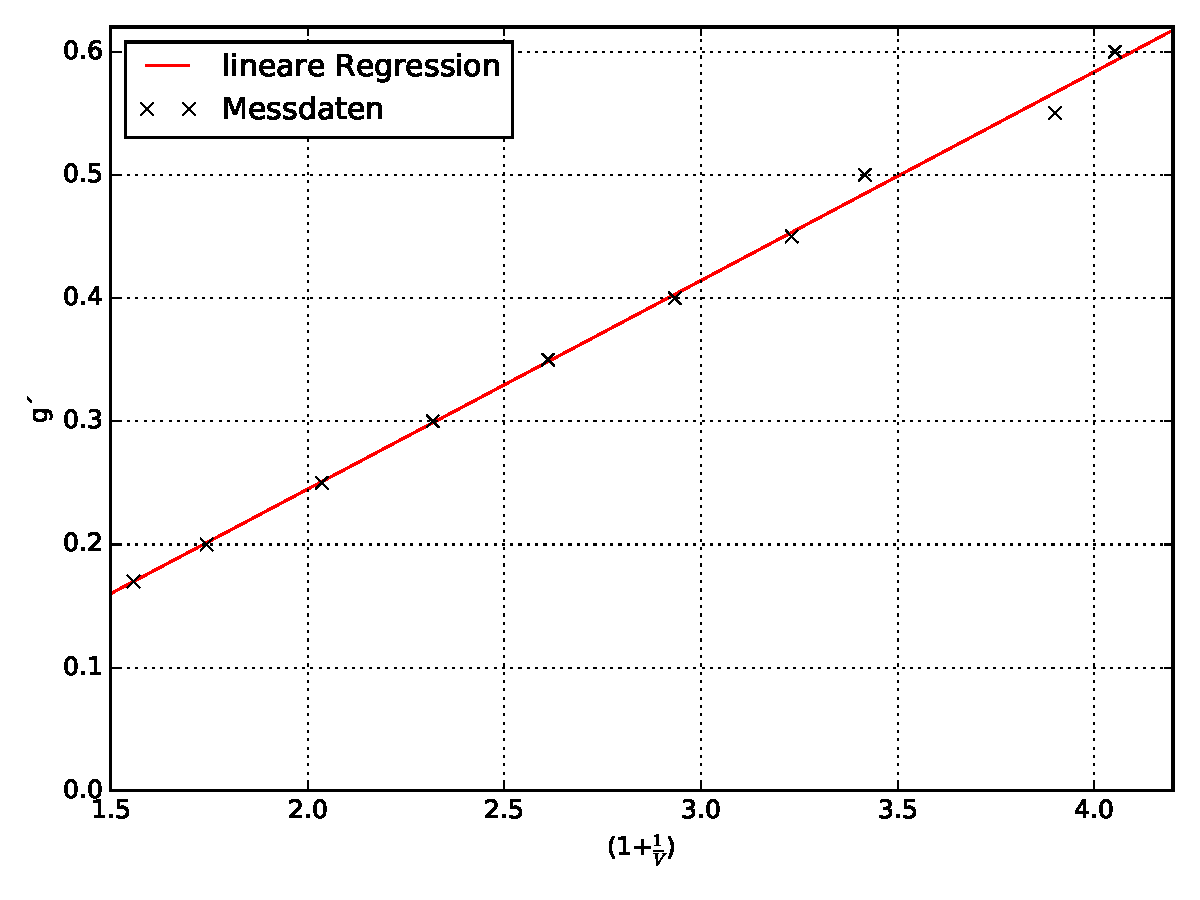
\includegraphics[width=\textwidth]{Pics/Messung_abbe_g.pdf}
  \caption{Wertepaare $(1 + \frac{1}{V_i}|g_i)$ mit linearer Regression.}
  \label{fig:abbe_g}
\end{figure}

\begin{figure}
  \centering
  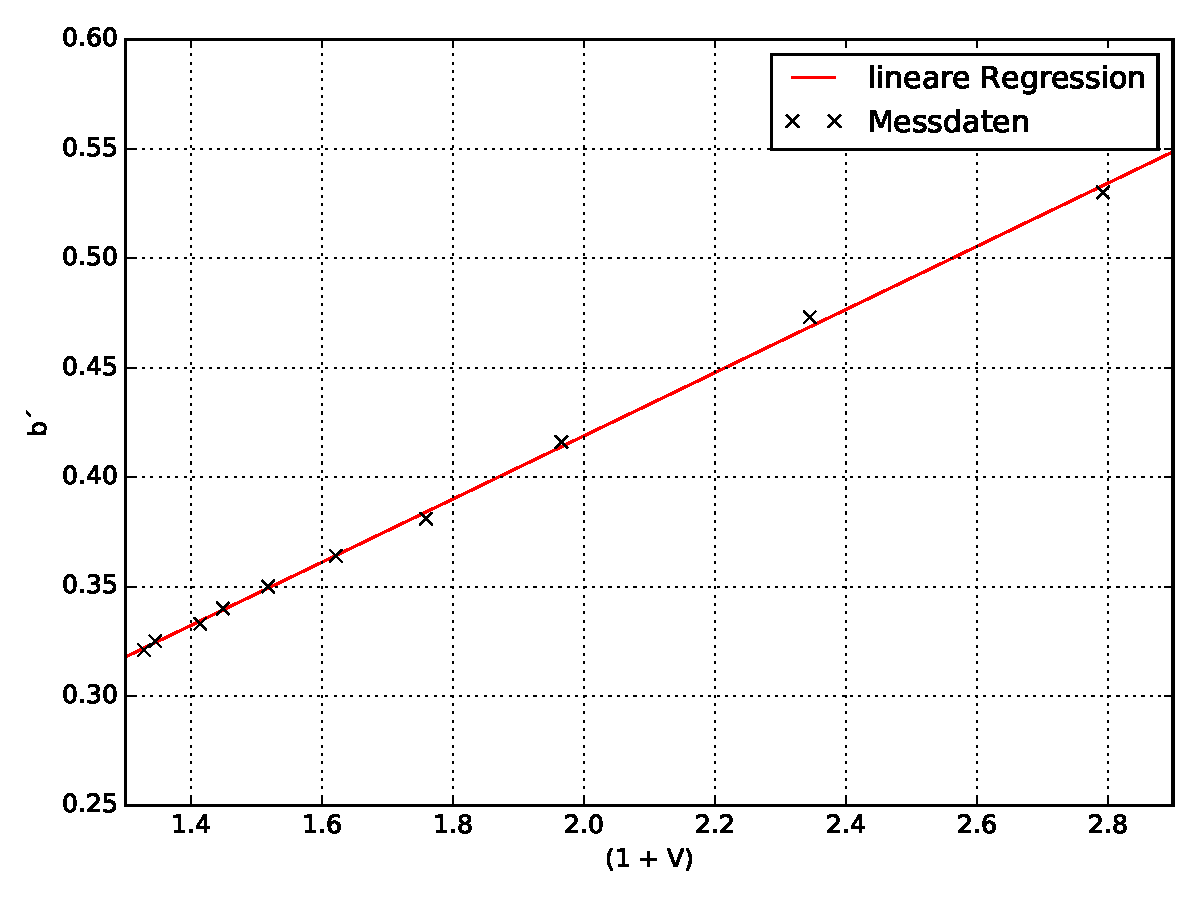
\includegraphics[width=\textwidth]{Pics/Messung_abbe_b.pdf}
  \caption{Wertepaare $(1 + V_i|b_i)$ mit linearer Regression.}
  \label{fig:abbe_b}
\end{figure}

\begin{table}
\centering
\caption{Messdaten der Methode nach Abbe}
\label{tab:abbe}
\begin{tabular}{S S S S S S }
\toprule
{Bildgröße $B$ in $\si{\centi\meter}$} & {Fehler $B$} & {$b + g$ in $\si{\centi\meter}$} & {Fehler $g + b$} & {$g$ in $\si{\centi\meter}$} & {Fehler $g$} \\
\midrule
 5.2  & 5.00  & 70.0  & 5.00  & 17  & 5.00\\
3.9  & 5.00  & 67.3  & 5.00  & 20  & 5.00\\
2.8  & 5.00  & 66.6  & 5.00  & 25  & 5.00\\
2.2  & 5.00  & 68.1  & 5.00  & 30  & 5.00\\
1.8  & 5.00  & 71.4  & 5.00  & 35  & 5.00\\
1.5  & 5.00  & 75.0  & 5.00  & 40  & 5.00\\
1.3  & 5.00  & 79.0  & 5.00  & 45  & 5.00\\
1.2  & 5.00  & 83.3  & 5.00  & 50  & 5.00\\
1.0  & 5.00  & 87.5  & 5.00  & 55  & 5.00\\
0.9  & 5.00  & 92.1  & 5.00  & 60  & 5.00\\
\bottomrule
\end{tabular}
\end{table}


Die Messgrößen in der Tabelle \ref{tab:abbe} haben alle den Ablesefehler
von $\SI{0,05}{\centi\meter}$

\section{Diskussion}

Anfangs ist zu erwähnen, dass der Grad der Bildschärfe per Hand, und somit
nur subjektiv bestimmt werden konnte. Damit ist anzunehmen, dass die Messergebnisse
auf Grund des Messverfahrens fehlerbehaftet sind.

Die Messgenauigkeit der Brennweitenmessung ist in Diagramm
\ref{fig:brennweite_bekannt} einzusehen. Bei einer hohen Messgenauigkeit haben
die eingetragenen Geraden einen gemeinsamen Schnittpunkt. Dies ist unter
Berücksichtigung der Messunsicherheit, erreicht worden. Die Messergebnisse
sind als präzise einzustufen.
Die Messergebnisse dieser Messung werden gemeinsam mit der Besselmethode
weiter unten diskutiert.

Das Abbildungsgesetz nach \eqref{eqn:Abbildungsgesetz} wurde ebenfalls
untersucht. Die Messungen \eqref{eqn:B/G} und \eqref{eqn:b/g} ergaben Werte,
die um ca. $\SI{2,6}{\centi\meter}$ voneinander abweichen. Die Werte sind nicht durch
den statistischen Fehler zu erklären und beruhen auf der Messmethode.
Die Bildgröße wurde mit einem Lineal vermessen und es ist anzunehmen,
dass der Ablesefehler sogar größer ist als der angenommene Ablesefehler.
Zudem trägt die anfangs erwähnte subjektive Einschätzung der Bildschärfe
zu der Abweichung bei.

Als Linse mit unbekannter Brennweite wurde eine befüllbare Linse genommen. Über eine
Spritze mit Wasser konnte die Befüllung der Linse reguliert werden.
Damit in der Linse ein konstanter Druck gewährleistet wurde, musste die Spritze an
einer definierten Position fixiert werden.
Die Fixierung wurde per Hand bewerkstelligt. Da das Messintervall relativ lang
war, konnte ein konstanter Druck über den gesamten Messzeitraum nicht
garantiert werden. Dadurch könnte
die Messung beeinflusst worden sein. Die Messung ergab eine Brennweite von
$f_2 = \SI{8,383(9)}{\centi\meter}$. Der in Diagramm
\ref{fig:unbekannte_brennweite} entstandene Schnittpunkt weißt hingegen auf eine
hohe Messgenauigkeit hin. Der Schnittpunkt der Geraden liegt bei $S_2 =
(\num{8,1(3)}|\num{8,4(3)})$.
Aus dem Mittelwerte der $x$- und der $y$-Koordinate ergibt sich eine
Brennweite von $\SI{8,25(30)}{\centi\meter}$.
Die beiden Brennweiten aus den verschiedenen Methoden der Brennweitenbestimmung
stimmen im Rahmen der Messungenauigkeit überein.

Die Messung der Linse mit unbekannter Brennweite ergab eine Brennweite von ca. $\SI{9,03}{\centi\meter}$.
Die Messgenauigkeit ist in Abbildung \ref{fig:unbekannte_brennweite} einzusehen.
Anhand des Schnittpunktes der Verbindungsgeraden ist die Messgenauigkeit im Rahmen
der Messung als präzise zu bewerten.

Mit der Methode nach Bessel wurde eine Brennweite von $f\ua{Bessel} =
\SI{9,67}{\centi\meter}$ festgestellt. Die Messung zur Überprüfung von
\eqref{eqn:Linsengleichung} ergab eine Brennweite von $f_1 =
\SI{9,525(9)}{\centi\meter}$. Die Abweichung der beiden Werte ist
hinsichtlich der Messgenauigkeit maginal. Die graphische Methode, die den
Schnittpunkt der Abb. \ref{fig:brennweite_bekannt} als Brennweite
angibt, ergab eine Brennweite von $\approx \SI{9,65(3)}{\centi\meter}$.
Dieser Wert ergibt sich aus dem Mittelwert der $x$- und $y$- Koordinate
des Schnittpunktes. Dieser Wert stimmt ebenfalls im Rahmen der
Messungenauigkeit mit den Brennweiten der vorigen Methoden überein.
Die bestimmten Brennweiten der verwendeten Linse weichen nur um $\approx\SI{0,5}{\centi\meter}$
von der Herstellerangabe ab. Daher sind die Messungen als präzise zu bewerten.

Die chromatische Abberration ergab, dass die Brennweite bei blauer Lichtquelle
minimal kleiner ist, als bei roter Lichtquelle. Die Werte weichen aber nicht
signifikant voneinander ab, sodass keine Aussage über die chromatische
Abberation gemacht werden kann.

Die Messung nach Abbe ergab eine Abweichung von
$\approx\SI{1}{\centi\meter}$ vom theoretischen Wert. Die Abweichung lässt
sich nicht durch den statistischen Fehler erklären und ist vermutlich
auf die verwendete Genauigkeit der Messmethode zurückführen. Zudem ist die Angabe des Herstellers
zu hinterfragen, welche bei den Rechungen des theoretischen Wertes als fehlerfrei
angenommen wurde.
